\documentclass[10pt,fleqn]{article} % Default font size and left-justified equations
\usepackage[%
    pdftitle={SLCI : Transformée de Laplace},
    pdfauthor={Xavier Pessoles}]{hyperref}
    \usepackage{import}
\subimport{../../../../style/}{preambule.tex}
%\fichetrue
\fichefalse
\proftrue
%\proffalse
%\tdtrue
\tdfalse
\courstrue
%\coursfalse
\subimport{../../../../style/}{new_style}
\subimport{../../../../style/}{macros_SII}
\subimport{../../../../style/}{preambule_trou.tex}

\usepackage{siunitx}
% -------------------------------------
% Déclaration des titres
% -------------------------------------

\def\discipline{Enseignement \\Technologique \\ Transversal}
\def\xxtete{Enseignement Technologique Transversal}

\def\classe{1 STI2D}
\def\xxnumpartie{Seq 3}
\def\xxpartie{Alimenter un système en énergie}

\def\xxnumchapitre{Séance 1}
\def\xxchapitre{\hspace{.12cm} La fonction alimenter/stocker}

\def\xxposongletx{2}
\def\xxposonglettext{1.45}
\def\xxposonglety{23}
\def\xxonglet{Seq. 3 -- Se. 1}

\def\xxactivite{Cours}
\def\xxauteur{\textsl{Geoffrey Vaquette}}

\def\xxcompetences{%
\textsl{%
\textbf{Savoirs et compétences :}
\begin{itemize}[label=\ding{112},font=\color{ocre}]
\item CO2.1	Identifier les flux et la forme de l'énergie, caractériser ses transformations et/ou modulations et estimer l'efficacité globale d'un système.
\end{itemize}
%
}}

\def\xxfigures{
\begin{center}
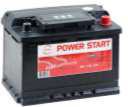
\includegraphics[width=2cm]{images/batterie.png} \\
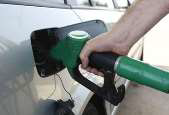
\includegraphics[width=2cm]{images/essence.png} \\
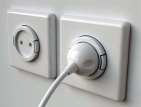
\includegraphics[width=2cm]{images/prise.png} \\
\end{center}
}%figues de la page de garde
\def\xxpied{%
La fonction alimenter/stocker \xxactivite%
}

%---------------------------------------------------------------------------

\renewcommand{\RemplirTrou}{false}
\begin{document}
\chapterimage{images/stockage_energie.jpg}
\subimport{../../../../style/}{new_pagegarde}
\section{Généralités}
\subsection{Définition}
Tout système nécessite de l’énergie pour fonctionner (pour agir sur la matière d'oeuvre). Dans la chaîne d’énergie, la fonction qui permet de fournir l’énergie est la fonction « Alimenter/Stocker ».

Nous nous intéresserons particulièrement dans ce cours à ce premier bloc de la chaîne d'énergie.

\begin{defi}
    Les éléments du bloc \textbf{Alimenter/Stocker} ont pour fonction de fournir l'énergie au système. Cette énergie peut provenir de l'extérieur du système (Réseau électrique par exemple) ou être stockée au sein du système (Batterie électrique par exemple).
\end{defi}


\subsection{Pourquoi stocker de l'énergie ?}
Le stockage de l'énergie est utilisé pour répondre à trois besoins principaux :
\begin{description}
    \item[Autonomie : ] Rendre un système mobile, capable de se déplacer avec sa source d'énergie.
    \begin{itemize}
        \item Voitures
        \item Téléphones
        \item Avion
        \item \dots
    \end{itemize}
    \item[Décalage temporel : ] Il n'est pas toujours possible de générer de l'énergie au moment où elle doit être utilisée. Par exemple, une maison équipée en panneau solaire ne pourrait pas être éclairée la nuit sans stockage de l'énergie.
    \item[Compensation des fluctuations : ]Il peut exister des fluctuations de courant électrique non désirées. Ces fluctuations peuvent être compensées par une réserve d'énergie.
\end{description}

\section{Stoker de l'énergie électrique}
L'énergie électrique est l'énergie la plus utilisée par l'être humain dans la société actuelle. Cette énergie provient de centrales à énergie renouvelables, ou non-renouvelables.

Il est aujourd'hui \textbf{impossible} de stocker de l'énergie sous forme électrique. Pour stocker cette énergie, il est donc indispensable de la convertir.

\subsection{Stockage chimique : piles et batterie}
Les piles et les batteries sont les principaux dispositifs que nous côtoyons au quotidien pour stocker de l'énergie.
L'énergie électrique est stockée dans des piles sous forme d'énergie chimique. Ces composants ont un coup abordable mais souvent un impact environnemental relativement fort.

\subsubsection{Caractéristiques des piles et batteries}
Les batteries sont caractérisées par trois grandeurs principales :
\begin{description}
    \item[La tension :] Classiquement notée $U$, la tension d'une batterie est la différence de potentiel qu'elle impose à ses bornes lors de sa décharge. Elle s'exprime en \textbf{volts (V)}

    \item[La capacité : ] C'est la quantité d'électricité (ou nombre de charges) stockée dans la batterie. Elle est habituellement indiquée en \textbf{ampère-heure (Ah)} ou en \textbf{Coulomb (C)}.

    \item[La densité énergétique : ]C'est la quantité d'énergie par unité de masse ou de volume. Elle s'exprime en \si{\frac{Wh}{kg}} ou \si{\frac{Wh}{L}}

\end{description}

\begin{table}[]
    \centering
    \begin{tabular}{>{\centering\arraybackslash} m{3cm}|>{\centering\arraybackslash} m{2cm}|>{\centering\arraybackslash} m{2cm}|>{\centering\arraybackslash} m{2cm}|>{\centering\arraybackslash} m{6cm}}
        \textbf{Type de batterie} & \textbf{Densité (\si{Wh/kg})} & \textbf{Plage de puissance} & \textbf{Rendement} & \textbf{Utilisation}  \\\hline
        Plomb & 50 & \SI{100}{W} à \SI{10}{MW} & 70 à 85 \% & \begin{itemize}
            \item Véhicules routiers électriques
            \item Sites non raccordés au réseau
        \end{itemize}\\\hline
        NiCd : Nickel-Cadmium& 50&Quelques Watts&70 à 80\%&\begin{itemize}
            \item Outillages portatifs
            \item Rasoirs électriques
        \end{itemize}\\\hline
        NiMH : Nickel Métal Hydrure&75&Quelques Watts&70 à 80\%&\begin{itemize}
            \item Téléphones portables
            \item Appareils photos
            \item Rasoirs électriques
        \end{itemize} \\\hline
        Li-ion : Lithium-ion&300&50W à 10MW&85 à 90\%& \begin{itemize}
            \item Téléphones portables
            \item Véhicules électriques
            \item Appareils photo
            \item Ordinateurs portables
        \end{itemize}\\\hline
        Li-Pol : Lithium-Polymère&120&100W à 10MW&85 à 90\%&\begin{itemize}
            \item Téléphones portables
            \item Véhicules électriques légers
        \end{itemize}
    \end{tabular}

    \caption{Quelques technologies de batteries.}
    \label{tab:my_label}
\end{table}

\begin{warn}
    Attention, il est important de ne pas confondre l'intensité (en \si{A}) et la capacité (en \si{Ah}).
\end{warn}

\begin{warn}
    La capacité d'une batterie ne représente pas directement la quantité d'énergie qu'elle contient. Pour connaître la quantité d'énergie contenue dans une batterie, il faut \textbf{multiplier sa capacité par sa tension} $$E = C \times U$$.
\end{warn}

\begin{rem}
        Une batterie contenant 10Ah sera capable de fournir un courant de 10A pendant 1h, ou encore un courant de 5A pendant 2h.
\end{rem}

\begin{exemple}
    Calculer la quantité d'énergie contenue dans une batterie d'une tension de $U = \SI{3}{V}$, d'une capacité de $Ca=\SI{1.5}{Ah}$.
\end{exemple}
\begin{correction}
     \trou{Une capacité de $C_a= \SI{1.5}{Ah}$ équivaut à une quantité de charges $q = Ca \times 3600 = \SI{5400}{C}$}
\end{correction}

\subsubsection{Association de batteries}

\begin{figure}[h]
    \centering
    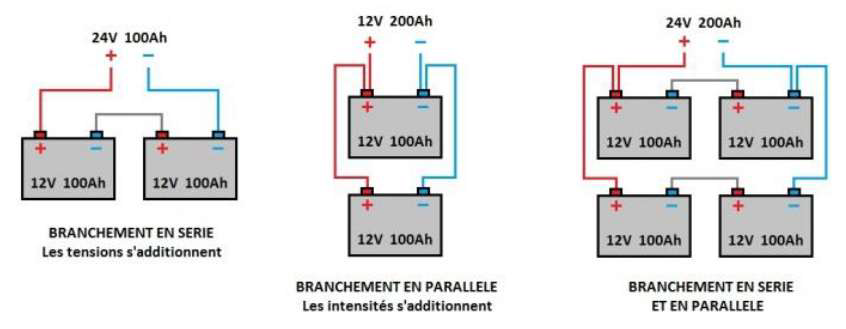
\includegraphics[width=\textwidth]{images/association.png}
    \caption{Association de batteries}
    \label{fig:association}
\end{figure}


\subsubsection{Synthèse : }
    \begin{aretenir}~
            \begin{itemize}
                \item Un courant électrique est un déplacement de charges (électrons).
                \item La quantité d'électricité $q$ (en coulomb \si{C}) est le produit de l'intensité \textbf{I} en \si{A} par le temps \textbf{t} en \si{s}.
                \item On peut également exprimer une quantité d'électricité $q$ en Ampère-heure (\si{Ah}).
            \end{itemize}
            \vspace{0.2cm}
        ~\hfill\fbox{\large$q = I\times t$}\hfill\fbox{\large$\SI{1}{Ah} = \SI{3600}{C}$}\hfill~
    \end{aretenir}

    \begin{aretenir}
        La puissance consommée $P$ en \si{W} est égale au produit de la tension \textbf{U} (en \si{V})  par le courant \textit{I} (en A) qui circule.

        \begin{center}
            \fbox{\large$P = U\times I$}
        \end{center}

    \end{aretenir}

    \begin{aretenir}
        L'énergie $E$ fournie par une batterie est :
        \begin{itemize}
            \item égale au produit de la \textbf{puissance absorbée} (en \si{W}) par le \textbf{temps de fonctionnement}
            \begin{itemize}
                \item Si t est en secondes \si{s}, E est en \si{J}
                \item Si t est en heures \si{h}, E est en \si{Wh}
            \end{itemize}
            \begin{center}
                \fbox{\large$E = P \times t$}
            \end{center}

            \item égale au produit de la capacité de la batterie par la tension ($\si{Ah}\times\si{V} = Wh$:
            \begin{center}
                \fbox{$E=C\times U$}
            \end{center}
        \end{itemize}
    \end{aretenir}

    \subsection{Stockage hydrolique}

    A plus grande échelle, on stocke de l'eau à l'aide de bassins de rétention :
    \begin{itemize}
        \item Lorsque l'on produit globalement plus d'énergie que la demande, on actionne des pompes pour faire monter l'eau dans un bassin en altitude.
        \item Lorsque l'on produit globalement \textbf{moins} d'énergie que la demande, on produit de l'électricité en faisant descendre l'eau dans des conduites pour activer des turbines.
    \end{itemize}

    \begin{figure}[h]
        \centering
        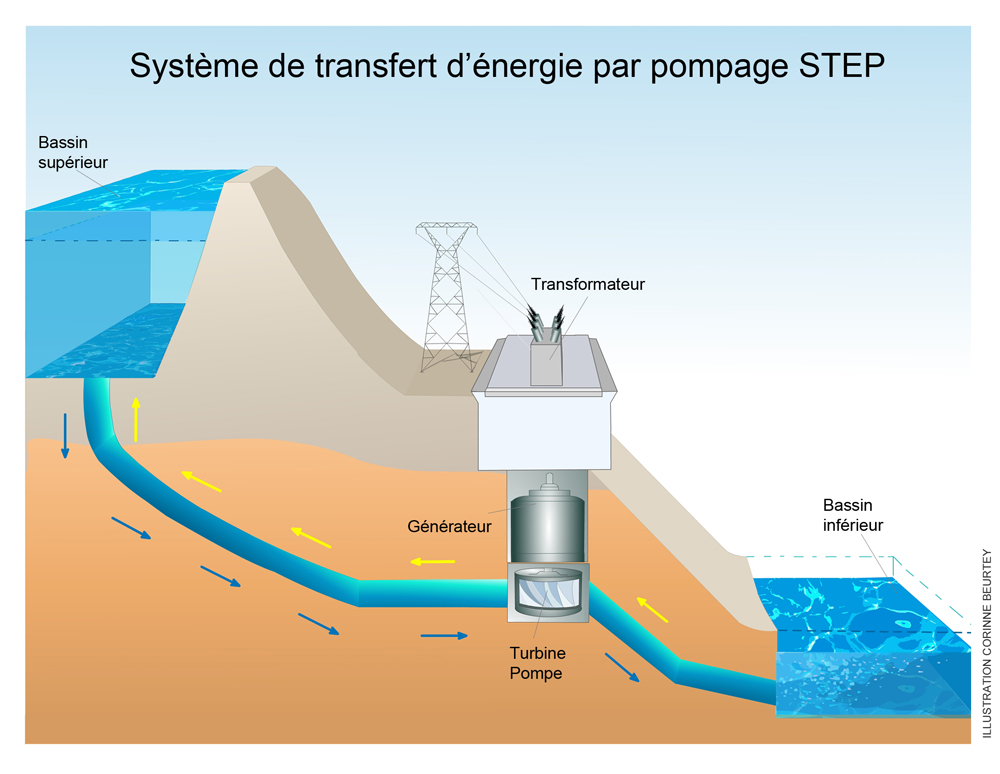
\includegraphics[width=\textwidth]{images/hydrau}
        \caption{Système de stockage d'énergie}
        \label{fig:hydrau}
    \end{figure}


    \section{Les signaux électriques}
    L'énergie électrique peut circuler sous différentes formes de signaux. Nous décrivons dans cette section les caractéristiques d'un signal électrique.

    \subsection{Les signaux périodiques}

    \begin{defi}
        Un signal est dit périodique si les variations de son amplitude se reproduisent régulièrement au bout d'une période \textbf{T} constante.

        \begin{center}
            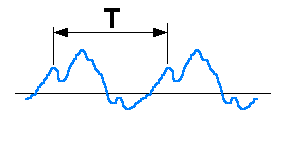
\includegraphics[width=0.3\textwidth]{images/Signal_periodique.png}
        \end{center}

        On a u(t+T) = u(t)
    \end{defi}

    \subsubsection{Caractéristiques d'un signal périodique}
    \begin{aretenir}~
    \begin{description}
        \item[La période T :] C'est la durée entre deux instants où la grandeur se reproduit identiquement à elle-même. La période s'exprime en \si{s}.

        \item[La fréquence f :] C'est le nombre de périodes présentes dans chaque seconde. Elle s'exprime en \si{Hz} est vaut :
        \begin{center}
            \fbox{$f = \frac{1}{T}$}
        \end{center}
        \item[Les valeurs maximales $S_{\text{max}}$ et minimales $S_{\text{min}}$] sont respectivement le maximum et le minimum du signal.
        \item[L'amplitude crête à crête $S_{CC}$] est l'écart entre les valeurs maximale et minimale : \fbox{$S_{CC} = S_{\text{max}} - S_\text{min}$}
        \item[L'amplitude A :] \fbox{$A = \frac{S_{CC}}{2}$}
        \item[Valeur efficace $S_\text{eff}$ : ] Elle est égale à la tension continue qu'il faudrait appliquer à une lampe pour qu'elle ait la même luminosité qu'avec une tension périodique.
    \end{description}
    \end{aretenir}

    \subsubsection{Le signal sinusoïdal}
    Le signal sinusoïdal est le type de signal le plus répandu dans les réseau électrique. Il a la forme d'une sinusoïde : $S = A\sin{\omega t} + S_\text{moy}$

    \begin{center}
        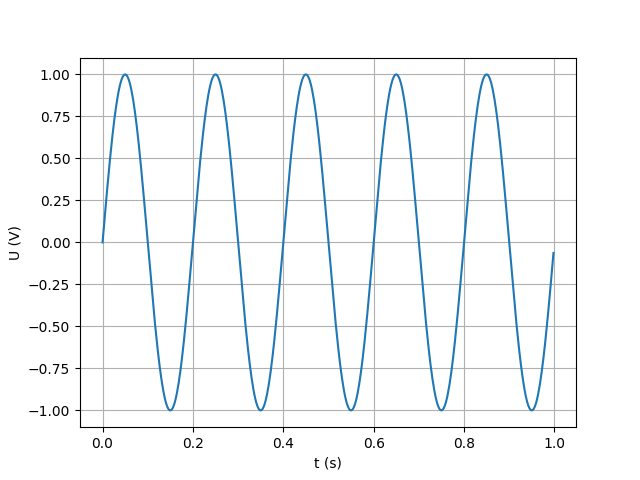
\includegraphics[height=0.3\textheight]{images/sinus.png}
    \end{center}
    \begin{itemize}
        \item La période de ce signal vaut : \trou{$T = \SI{0.2}{s}$}
        \item La fréquence de ce signal vaut : \trou{$f = \frac{1}{T}\SI{5}{Hz}$}
        \item  L'amplitude de ce signal vaut : \trou{$A = 1V$}
    \end{itemize}




    \subsubsection{Le signal carré}
    Un signal carré est généralement employé pour transporter une information ou pour commander un moteur à courant continu.
    \begin{center}
        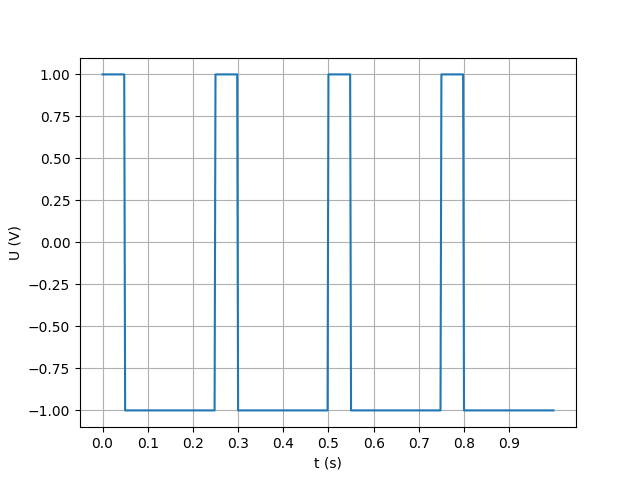
\includegraphics[height=0.3\textheight]{images/carre.png}
    \end{center}

    \begin{defi}
        Le rapport cyclique $\alpha$ d'un signal carré est le temps resté à l'état haut divisé par la période du signal.
    \end{defi}

    \begin{exemple}
        Le rapport cyclique de ce signal vaut : \trou{0.3}
    \end{exemple}


    \subsubsection{Le signal triangulaire}
    \begin{center}
        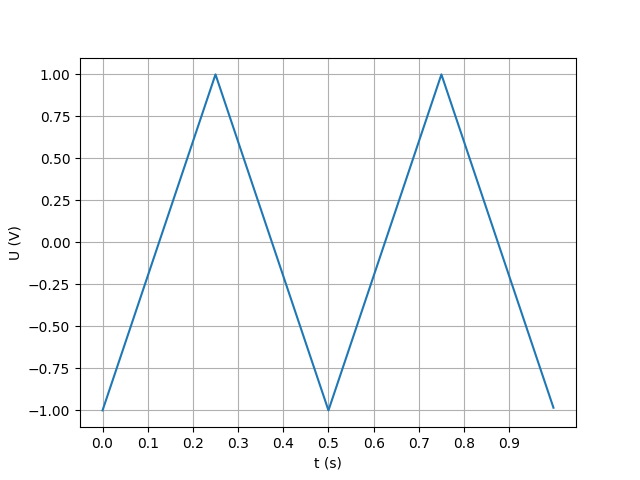
\includegraphics[height=0.3\textheight]{images/triangle.png}
    \end{center}

    \begin{itemize}
        \item La période de ce signal vaut : \trou{$T = \SI{0.2}{s}$}
        \item La fréquence de ce signal vaut : \trou{$f = \frac{1}{T}\SI{5}{Hz}$}
        \item  L'amplitude de ce signal vaut : \trou{$A = 1V$}
    \end{itemize}
    \pagebreak
    \section{Les appareils de mesures}
    \begin{figure}[h]
        \centering
        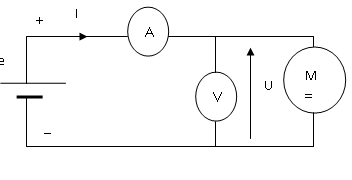
\includegraphics[height=0.2\textheight]{images/branchement.png}
        \caption{Branchement d'un voltmètre et d'un ampèremètre dans un circuit}
        \label{fig:branchement}
    \end{figure}

    \subsection{L'ampèremètre}
    L'ampèremètre sert à mesurer un courant électrique I. Il se place en \textbf{série} dans le circuit.

    \subsection{Le voltmètre}
    Le voltmètre sert à mesurer une tension électrique (une différence de potentiel entre un point A et un point B du circuit). Il se place en dérivation entre A et B
\end{document}
